% !TeX root = ../main.tex
% Add the above to each chapter to make compiling the PDF easier in some editors.

\chapter{Introduction}\label{chapter:introduction}

\section{Applications of Microwave Imaging}
Finding information about an area of interest by measuring certain physical properties from this area at one or more places is a fundamental problem.
After all, the human senses (sight, hearing, touch, smell, taste) are all measurements of the environment to recreate a model of the world around us.
Usually the processed information is visualized in a way that is easy to understand for humans, these algorithms are called imaging algorithms.
In electromagnetic (EM) imaging, the goal is to reconstruct the properties of an object from measurements of the scattered electromagnetic field.
This problem is called the inverse-scattering problem.
In some sense our eyes are also an EM imaging system, as they measure the light  which is scattered by the surrounding objects it hits.
The applications of EM-imaging reach from medical imaging (MRI, CT) to security (metal detectors, concealed weapon detection) and geophysics (seismic imaging, ground-penetrating radar).
They vary mostly in the frequency of the used electromagnetic field, as this determines the penetration depth and the resolution of the imaging system.
The higher the frequency, the higher the resolution, but the lower the penetration depth.
This thesis focusses on waves in the microwave frequency range (around 300 MHz to 300 GHz) which corresponds to a wavelength of 1m to 1mm.
Waves of this wavelength will result in a scattering effect when hitting an object of similar size, so they are well suited for practical applications~\parencite{pastorino_microwave_2018}.
Microwave imaging is used in medical applications (breast cancer detection, brain imaging)~\parencite{wang_medical_2014}, security (contraband detection, people screening)~\parencite{ahmed_microwave_2021} and civil engineering (crack detection, subsurface inspection)~\parencite{pastorino_microwave_2018}.

\section{The Principle behind Time-Reversal Imaging}
Time-reversal imaging is about finding the cause of present measurements in the past.
This is can be illustrated by the example of three kids (A, B and C) playing catch with a ball.
Make a video of kid A throwing the ball to kid B and then revert the video.
The video will then show, how the ball flies from kid B to kid A.
Anyone that is asked whether the ball was thrown by kid A or kid C after being shown the reverted video could conclude that it must have been kid A who threw the ball and not kid C.
This problem is trivial if a video of the whole setup and the whole process of throwing and catching the ball is available.
Now suppose, that the video only shows how kid B caught the ball.
Simply time-reverting this video will not reveal who threw the ball in the first place.
But if kid B would exactly replicate the movement in the time-reversed video, it would throw the ball back where it came from so it would land at kid A.
This is the principle behind any time-reversal imaging algorithm.
Its application to microwave imaging is more complex, as the impact of the source doe not spread into one single direction like the ball, but as a wave into all directions.
It shows one of the main flaws of time-reversal imaging, namely that for it to work it is necessary to measure the whole impact of the source.
In case of the player throwing a ball this was easy, as the whole impact is bound to the ball.
A wave on the other hand will propagate in all directions, so there would have to be measurements all around the setting.
Figure~\ref{fig:WaveTimeReversal} shows a receiver array around the source measuring an expanding wave.
The measured signal is then re-emitted by the receivers and contracts at the source location, creating an approximated version of the time-reversed expanding wave (see figure~\ref{fig:WaveTimeReversalContraction}).
If there were infinitely many receivers around the source, they would create a perfect time-reversed wave.

\begin{figure}[ht]
    \centering
    \begin{minipage}{0.45\textwidth}
        \centering
        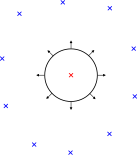
\includegraphics[width=\textwidth]{build/WaveExpanding.pdf}
        \caption{The wave coming from a source (red) is measured at some receivers (blue).}\label{fig:WaveTimeReversal}
    \end{minipage}\hfill
    \begin{minipage}{0.45\textwidth}
        \centering
        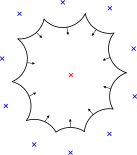
\includegraphics[width=\textwidth]{build/WaveContracting.pdf}
        \caption{The measured wave is re-emitted by the receivers and contracts at the source-location}\label{fig:WaveTimeReversalContraction}
    \end{minipage}
\end{figure}